% !TeX root = RJwrapper.tex
\title{Understanding pandoc lua filters}
\author{by Abhishek Ulayil}

\maketitle

\abstract{
pandoc supports intermediate modification of the Abstract Syntax Tree (AST) between
the parsing and writing phase using filters. This supplement paper will highlight
the use cases of such filters written in Lua Language on LaTeX,markdown and native AST.
}

\section{Introduction}
To understand pandoc filters, one must look at the document conversion process in
general. A document is read/parsed in one format to a common intermediate format.
In pandoc it is called an abstract syntax tree (AST). A document writer is designed 
to read the AST and write the contents in the form of desired article format.
For example converting markdown to HTML will involve these processes in pandoc.

\begin{figure}[htbp]
  \centering
  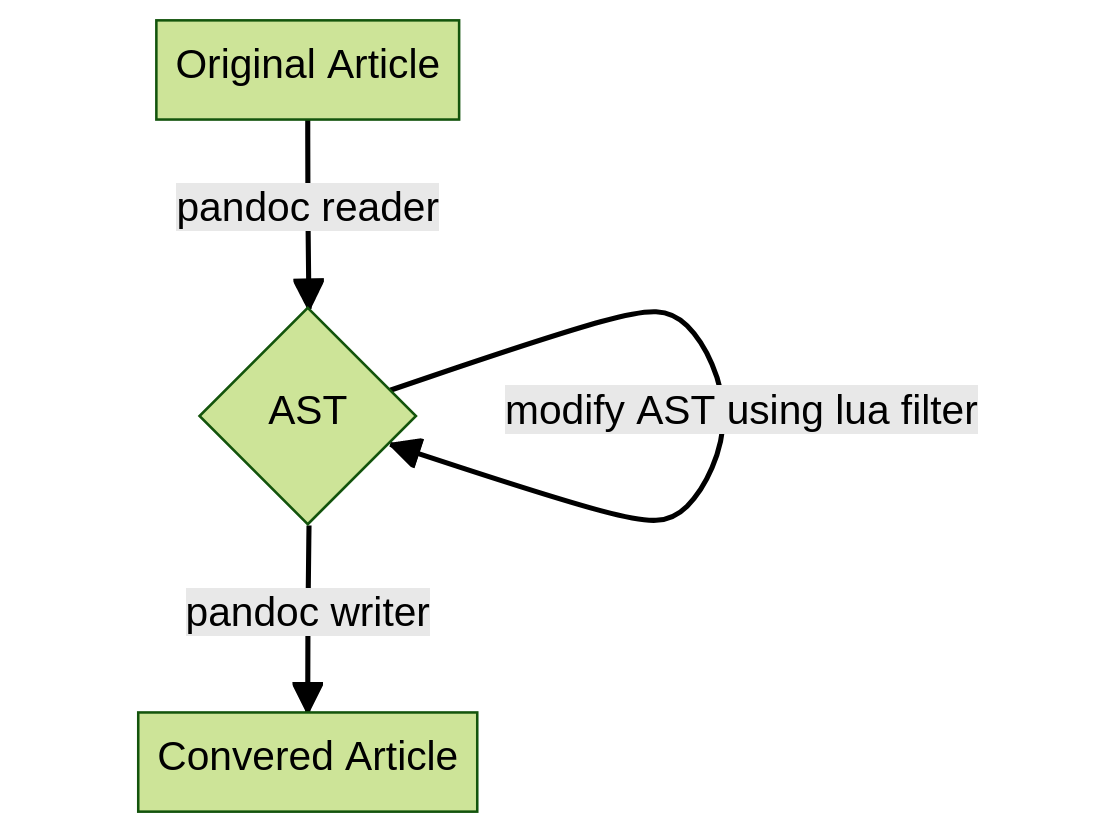
\includegraphics[width=0.6\textwidth]{workflow.png}
  \caption{Conversion Workflow}
  \label{fig:workflow}
\end{figure}

The filters come into picture when there are certain elements which require 
customization. For example, suppose you are converting markdown to HTML and you
require the page to have automatic numbering for figures or tables. 
If you think about it in markdown there is no system of numbering figures/tables 
automatically, to retain 1:1 conversion the HTML output will miss the numbering as well. 
At this moment you would wish that there was some option to add such a feature,
but then given the infinite possibilities of customization it is not feasible to 
add each and every customization as an option in pandoc or the writer. 
To tackle this, the idea of filters arrived, wherein you could manipulate the AST
partly or fully and modify it before the writer could read the AST. Hence generating
an output you desire \citep{pandocfilters}.

\section{Writing lua filters}

Continuing the example above lets create a dummy article, where we need to add
numbering. One way could be to keep a counter of Images, and add a prefix \verb|"Figure X :"|
to each figure caption. This will serve the purpose of numbering the Images in the end result.

\begin{verbatim}
![R logo](Rlogo-5.png){width="10%"}

![penguins](penguins.png){width="15%"}

\end{verbatim}

\begin{figure*}[htbp]
\begin{verbatim}
pandoc example.md --from markdown --to html5 --output example.html
\end{verbatim}
\caption{pandoc command without lua filter or extensions}
\label{code:2}
\end{figure*}

Now If we convert the above markdown file to HTML5 using pandoc command \ref{code:2}, we get \ref{fig:1}


\begin{figure*}[!htbp]
\centering

\includegraphics[width=0.5\linewidth]{example.png}
\caption{Vanilla HTML5 output}
\label{fig:1}
\end{figure*}

\section{Using pandoc lua filters}

As we can see, there is no figure numbering done automatically, which is generally
the expected result. However if we want to include numbering to it, we would need
to write a lua filter. This lua filter will modify the AST and make the changes we 
desire.

We call a lua filter in the pandoc command \ref{code:2} using the \verb| --lua-filter name_of_filter.lua|
option in pandoc.

Now we write a lua filter to manipulate the figures in \ref{code:3}
\subsection{TODO : explain lua filter in more detail.}
\begin{figure}[htbp]
\begin{verbatim}
figures = 0
is_fig = 0

function Figure(el)
      local label = ""
      pandoc.walk_block(el,{ Image = function(el)
                     is_fig = 1
                     end})
      if is_fig == 1 then
	        figures = figures + 1
	        label = "Figure " .. tostring(figures) .. ":"
      end
	    local caption = pandoc.utils.stringify(el.caption)
	    if not caption then
          caption = label
    	else
          caption = label .. " " .. caption
    	end
    	el.caption.long[1] = caption
    	is_fig = 0
    	return el
end
\end{verbatim}
\caption{A lua filter to add figure numbering}
\label{code:3}
\end{figure}

\section{Interpreting changes using lua filters}

The filter \ref{code:3} when included in the pandoc command will generate \ref{fig:2} 
using the \ref{code:4} command.

\begin{figure}[htbp]
\begin{verbatim}
pandoc example.md --from markdown --to html5 --output filtered-example.html
--lua-filter image_numbering_filter.lua
\end{verbatim}
\caption{pandoc command with lua filter}
\label{code:4}
\end{figure}

\begin{figure}[htbp]
\centering
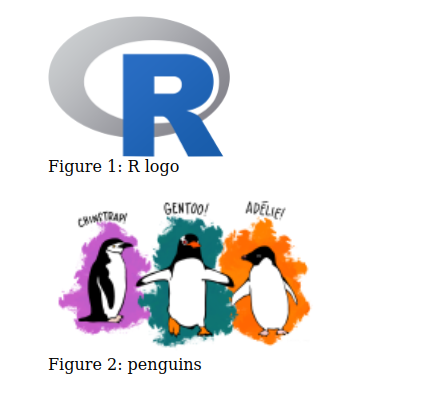
\includegraphics[width=0.5\linewidth]{example-filtered.png}
\caption{HTML5 output with desired filtering}
\label{fig:2}
\end{figure}

\section{Usage of pandoc lua filters in texor package}


\section{Summary}

\section{Supplementary materials}
The example conversion files described here are included as supplementary materials
in the Rjournal article of texor.

\begin{thebibliography}{2}
    \providecommand{\natexlab}[1]{#1}
    \providecommand{\url}[1]{\texttt{#1}}
    \expandafter\ifx\csname urlstyle\endcsname\relax
      \providecommand{\doi}[1]{doi: #1}\else
      \providecommand{\doi}{doi: \begingroup \urlstyle{rm}\Url}\fi

\bibitem[Krewinkel, Lucero (2023)]{pandoc}
A.~ Krewinkel and A.~ Lucero,
\newblock pandoc 3.0 Release notes,
\newblock \emph{pandoc} \penalty0 2023
\newblock URL \url{https://pandoc.org/releases.html#pandoc-3.0-2023-01-18}

\bibitem[MacFarlane and other pandoc authors (2023)]{pandocfilters}
John MacFarlane and other pandoc authors,
\newblock Pandoc Lua filters,
\newblock \emph{pandoc documentation} \penalty0 2023
\newblock URL \url{https://pandoc.org/lua-filters.html}

\end{thebibliography}


\address{%
Abhishek Ulayil\\
Student, Institute of Actuaries of India\\%
Mumbai, India\\
ORCiD: 0009-0000-6935-8690\\
}
